\documentclass{article}

\usepackage{graphicx}
\usepackage{tikz}
\usepackage{tikzsymbols}
\usetikzlibrary{calc,patterns,shapes.geometric}
\pagestyle{empty}
\usepackage[margin=0pt]{geometry}
\geometry{papersize={14in,12in}}

\def\centerarc[#1](#2)(#3:#4:#5){\draw[#1] ($(#2)+({#5*cos(#3)},{#5*sin(#3)})$) arc (#3:#4:#5);}

\begin{document}
	\begin{figure}
		\centering
		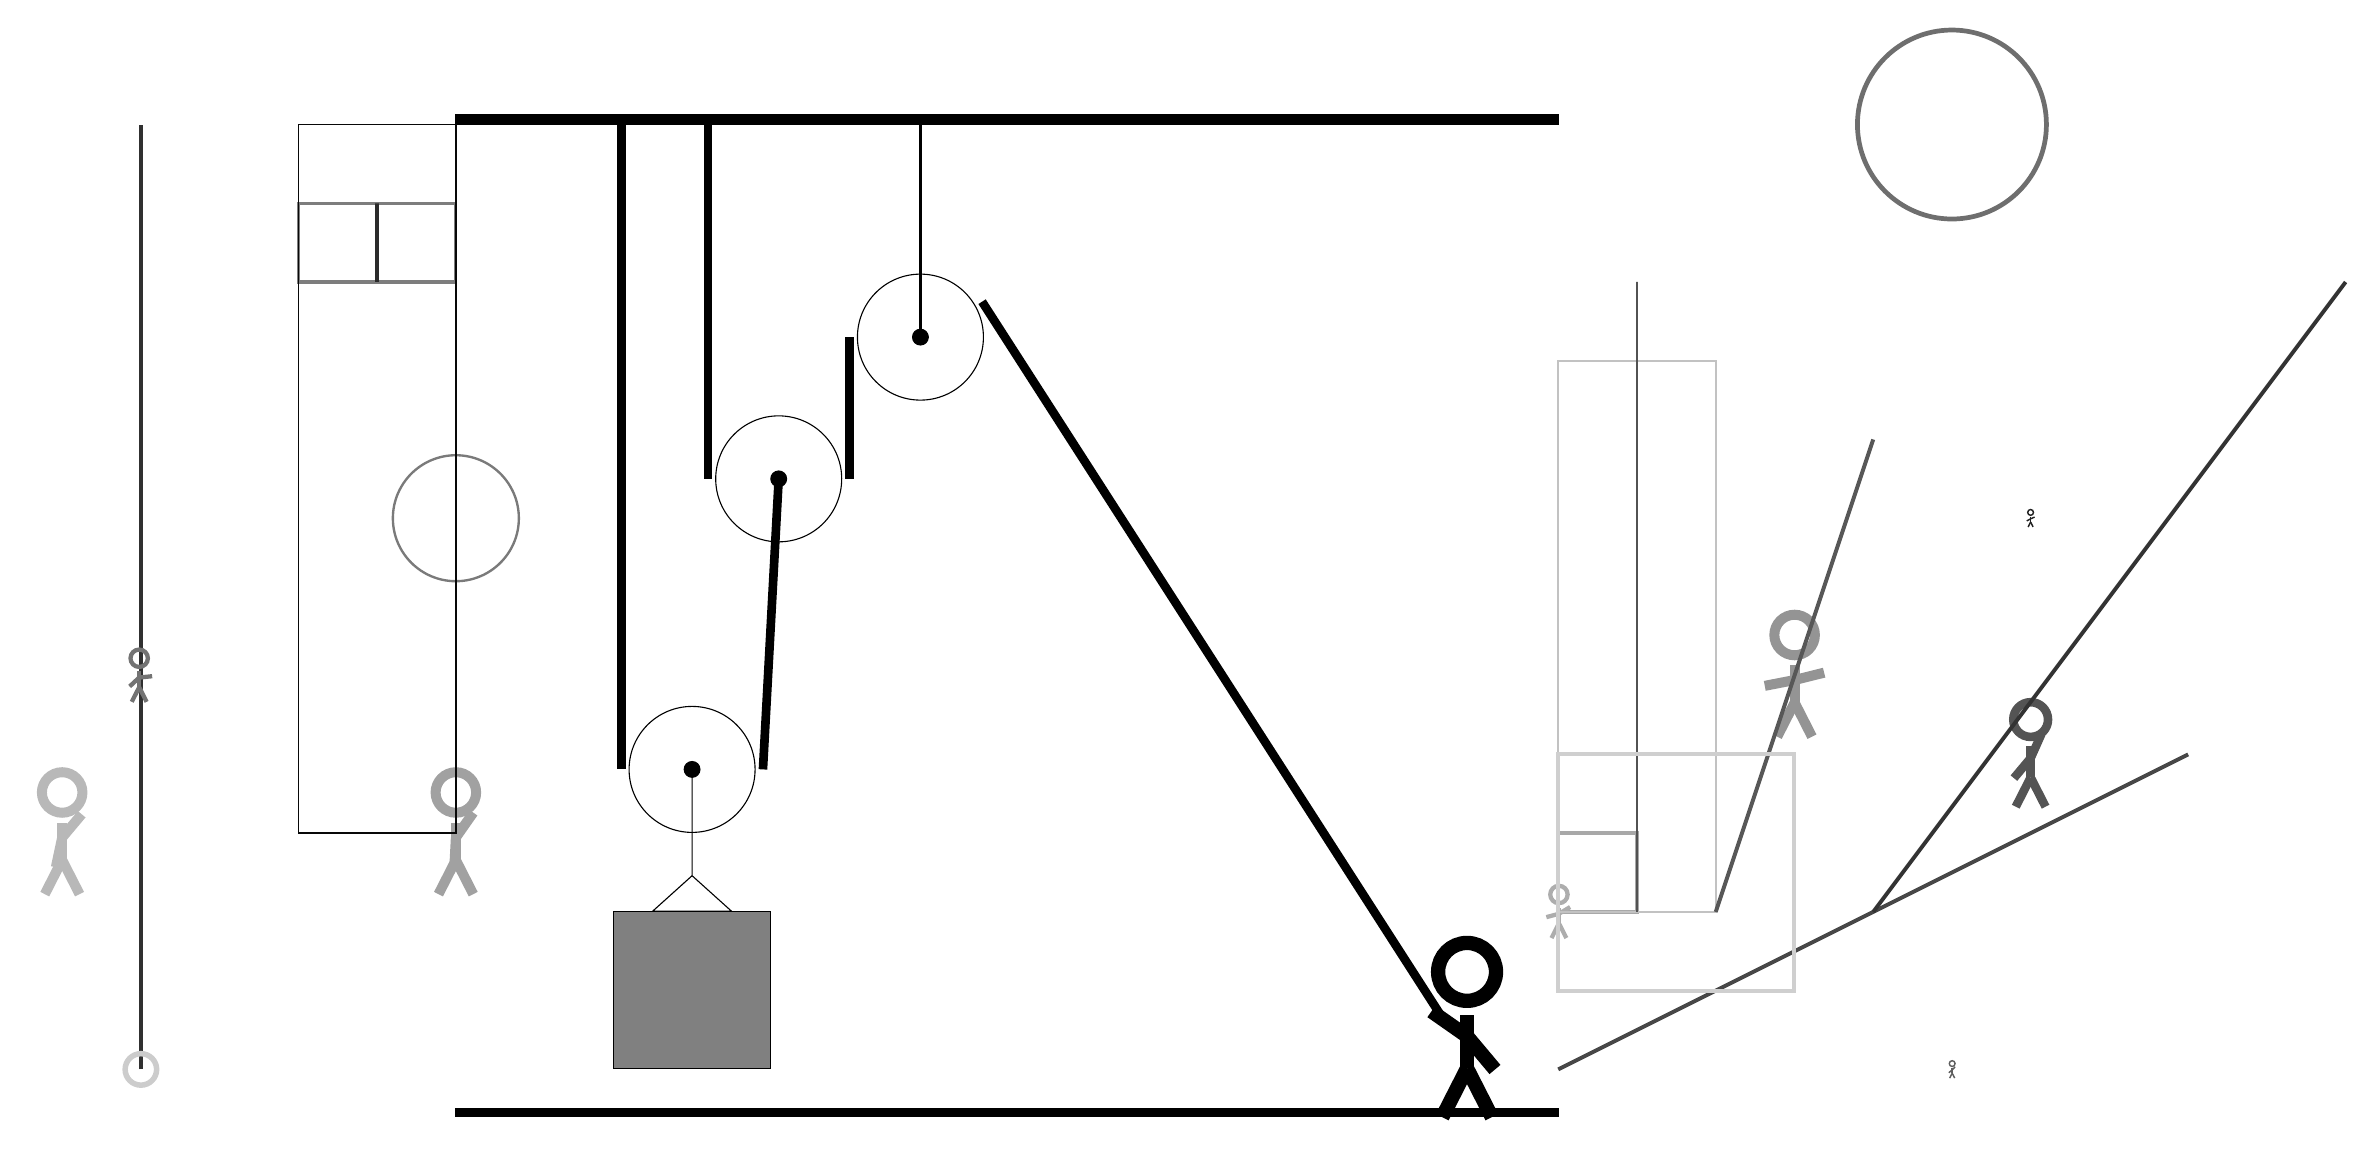
\begin{tikzpicture}
			%%%%% START %%%%%
			
			\draw[fill=black] (-2, 9) rectangle (12, 9.125);
			
			\draw (1, 0.81) circle (0.8);
			\draw[fill=black] (1, 0.81) circle (0.1);
			
			\draw (2.1, 4.5) circle (0.8);
			\draw[fill=black] (2.1, 4.5) circle (0.1);
			
			\draw (3.9, 6.3) circle (0.8);
			\draw[fill=black] (3.9, 6.3) circle (0.1);
			\draw[thick] (3.9, 6.3) -- (3.9, 9);
			
			\draw[line width=0.4mm, color=black!51] (-2, 7) rectangle (-4, 8);
			
			\draw[line width=0.5mm, color=black!81](-6, -3) -- (-6, 9);
			\draw[line width=0.5mm, color=black!72](12, -3) -- (20, 1);
			\draw[line width=0.5mm, color=black!34] (12, -1) rectangle (13, 0);
			
			\node[line width=0.7mm, color=black!42] at (15, 2) {\Strichmaxerl[7][11][14]};
			
			\node[line width=0.3mm, color=black!32] at (12, -1) {\Strichmaxerl[3][15][31]};
			\draw[line width=0.5mm, color=black!83] (-3, 8) rectangle (-3, 7);
			
			\draw[line width=0.3mm, color=black!24] (12, -1) rectangle (14, 6);
			\draw [line width=0.6mm, color=black!57](17, 9) circle (1.2);
			\draw[line width=0.2mm, color=black!68] (13, 7) rectangle (13, -1);
			\node[line width=0.5mm, color=black!67] at (18, 1) {\Strichmaxerl[6][50][66]};
			\node[line width=0.7mm, color=black!63] at (17, -3) {\Strichmaxerl[1][38][48]};
			\node[line width=0.3mm, color=black!28] at (-7, 0) {\Strichmaxerl[7][78][50]};
			
			\draw [line width=0.7mm, color=black!20](-6, -3) circle (0.2);
			\node[line width=0.3mm, color=black!87] at (18, 4) {\Strichmaxerl[1][28][24]};
			\node[line width=0.7mm, color=black!37] at (-2, 0) {\Strichmaxerl[7][87][55]};
			
			\draw[line width=0.5mm, color=black!80](16, -1) -- (22, 7);
			\node[line width=0.2mm, color=black!55] at (-6, 2) {\Strichmaxerl[3][43][6]};
			\draw [line width=0.3mm, color=black!52](-2, 4) circle (0.8);
			
			\draw[line width=0.2mm, color=black!97] (-2, 9) rectangle (-4, 0);
			\draw[line width=0.5mm, color=black!66](16, 5) -- (14, -1);
			\draw[line width=0.5mm, color=black!19] (12, 1) rectangle (15, -2);
			
			\draw (1, 0.81) -- (1, -0.54) -- (0.5, -0.99) -- (1.5, -0.99) -- (1, -0.54);
			\draw[fill=black!50] (0, -0.99) rectangle (2, -2.99);
			
			\draw[line width=1.1mm] (0.1, 9) -- (0.1, 0.81);
			\centerarc[line width=1.1mm](1, 0.81)(180:360:0.9);
			\draw[line width=1.1mm](1.9, 0.81) -- (2.1, 4.5);
			\draw[line width=1.1mm] (1.2, 9) -- (1.2, 4.5);
			\centerarc[line width=1.1mm](2.1, 4.5)(180:360:0.9);
			\draw[line width=1.1mm](3.0, 4.5) -- (3.0, 6.3);
			\centerarc[line width=1.1mm](3.9, 6.3)(30:180:0.9);
			\draw[line width=1.1mm] (4.683, 6.75) -- (10.5, -2.3);
			
			\node at (10.8, -2.5) {\Strichmaxerl[10][-35][-50]};
			
			\draw[fill=black] (-2, -3.5) rectangle (12, -3.6);
			
			%%%%% END %%%%%
		\end{tikzpicture}
	\end{figure}	
\end{document}